The aLIGO interferometers are highly complex, high precision devices. 
Their operation depends on the careful interaction of a series of subsystems, 
each with its own purpose. In an effort to better understand the operation 
and output of the interferometers, the Detector Characterization group has 
been designed to mirror this subsystem approach. Table 
\ref{table:aligo-subsystems} lists the aLIGO subsystems. Each of these 
subsystems is assigned a data quality liaison from the DetChar group. 

\begin{table}[ht!]%
  \begin{center}
    \begin{tabular}{|c|l|}
    \hline
    Subsystem & Description \\
    \hline
    LSC & Length Sensing and Control \\
    \hline
    ASC & Alignment Sensing and Control \\
    \hline 
    SUS & Suspensions \\
    \hline
    IMC & Input Mode Cleaner \\
    \hline 
    OMC & Output Mode Cleaner \\
    \hline
    PCAL & Photometric Calibration \\
    \hline 
    PEM & Physical Environmental Monitoring \\
    \hline
    SEI & Seismic Isolation \\
    \hline
    PSL & Pre-Stabilized Laser \\
    \hline
    TCS & Thermal Compensation System \\
    \hline
    \end{tabular}
  \end{center}
  \caption[Table of aLIGO subsytems]{Table describing aLIGO subsystems}
  \label{table:aligo-subsystems}
\end{table}

There are 5 main responsibilities assigned to a subsystem liaison. The 
first is to fully understand the operation and installation of the subsystem 
so that they can faciliate data quality investigations and act as a 
point of contact for commissioners assigned to this subsystem.

The second responsibility 
is to take this knowledge and use it to populate the channel information 
system (CIS), which is a database that stores information about how to 
parse and understand the various auxiliary channels that are monitored 
in each subsystem. This database also contains information about calibration 
and valid frequency ranges for these channels. This allows newcomers to the 
collaboration to more easily familiarize themselves with the LIGO naming 
conventions and facilitates their involvement in data quality investigations.  

The third responsibility 
is to check for signal fidelity, which means to make sure that all of the 
channels are working as intended and don't contain artifacts from signal 
conditioning processes.

The fourth responsibility is to develop summary pages that monitor 
important channels and figures of merit for each subsystem. 
The summary pages are generated 
every day from a configuration file designed by the subsystem liaisons. 
The purpose of the summary pages is to gather all of the potentially 
useful information about a subsystem in an organized way so that the 
subsystem leads can efficiently evaluate the performance of the subsystem. 
They are also a useful launch point for data quality shifts and 
investigations since they provide various overviews of instrumental 
performance ($h(t)$ spectrograms, Omicron triggers, BNS inspiral range, etc.) 
that make it easy to identify persistent or egregious data quality issues.

The fifth and final responsibility is to develop and build real-time 
data quality monitors in the Online Detector Characterization (ODC) 
framework. 
The Online Detector Characterization (ODC) system is an infrastructure designed
to extract and record metadata describing the state of the aLIGO interferometers.
This state information has two main purposes: to inform data quality investigations
by the DetChar group and to serve as a real-time monitor of the interferometer state
that can be accessed in the control room. Each subsystem monitored by the DetChar group
using an ODC monitor.

The ODC system is unique in that it is runs in real-time in the front-end control
system that is used to control the aLIGO interferometers. Each set of ODC monitors
is built in Simulink to directly interface with the models that run on the front-end
computers. This has several distinct advantages.
Since the monitors are run in real-time, they operate in parallel with the control
loops that are sensing the various degrees of freedom of the interferometer and are
able to achieve highly precise timing. The ODC monitors can also create their own
test points, which means an ODC monitor can perform a check on any signal that exists
in the front end at its full rate instead of relying on the information that is
downsampled and stored in frames.
These full rate test points operate at the full sample rate of the model (16384 Hz)
and any information recorded in the ODC channel is written at the same rate. In contrast,
many channels are only recorded at 16 Hz if they aren't accessed as a test point in the front-end system.

The information generated by each ODC monitor can be extracted and sent to a segment
generation process, where the most useful information is catalogued and represented by
segments of time that indicate when a given flag was considered to be active.

\section{Length Sensing and Control}

The Length Sensing and Control (LSC) subsystem is 
used to monitor and control the lengths of the various optical cavities in the 
aLIGO interferometers. Figure (insert) shows the layout 
of the aLIGO interferometer with the lengths of individual optical cavities 
labeled. The LSC subsystem is responsible for controlling 5 global degrees of freedom, 
which are linear combinations of these individual cavity lengths. Table (insert) 
describes the primary degrees of freedom controlled by the LSC subsystem. 
This is a critical subsystem, as it is used to control
not only the auxiliary optical cavities, but the DARM degree of freedom which
is sensitive to gravitational wave signals.
These optical cavities are controlled using the Pound-Drever-Hall (PDH) 
technique.

\subsection{Length locking basics}

This is how a basic PDH loop works and where the error signals are picked 
off from.

\subsection{Online Detector Characterization}


Figure \ref{fig:lsc-odc-model} shows the implementation of an LSC ODC 
model in SIMULINK. 

\begin{figure}[ht!]
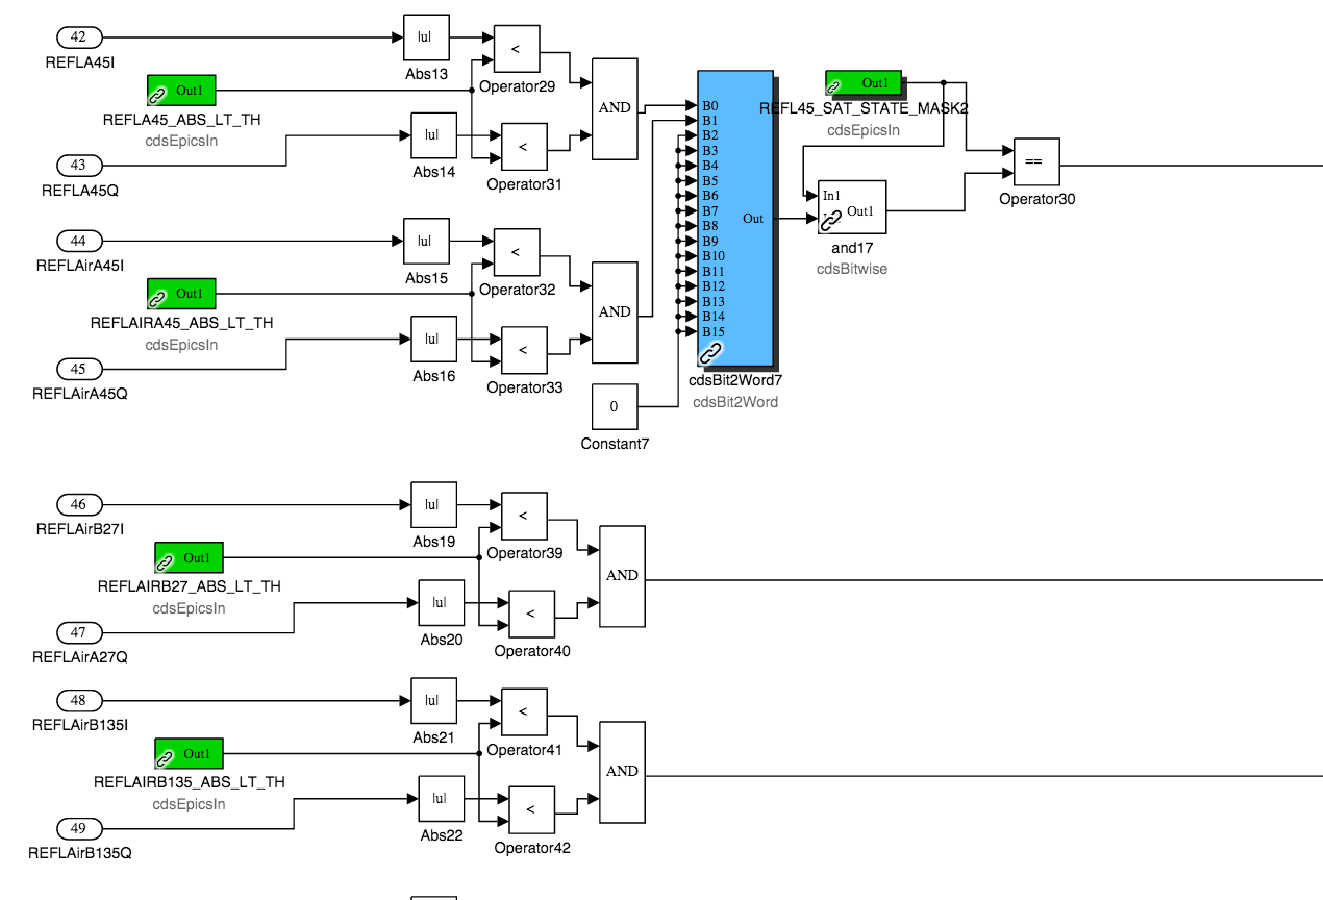
\includegraphics[width=\textwidth]{figures/ODC/LSC-ODC-model}
\caption[LSC ODC SIMULINK Model Example]{Example of LSC ODC bits implemented in SIMULINK}
\end{figure}\label{fig:lsc-odc-model}

\subsection{MEDM screens}

Figure \ref{fig:lsc-odc} shows the LSC ODC overview screen in MEDM.

\begin{figure}[ht!]
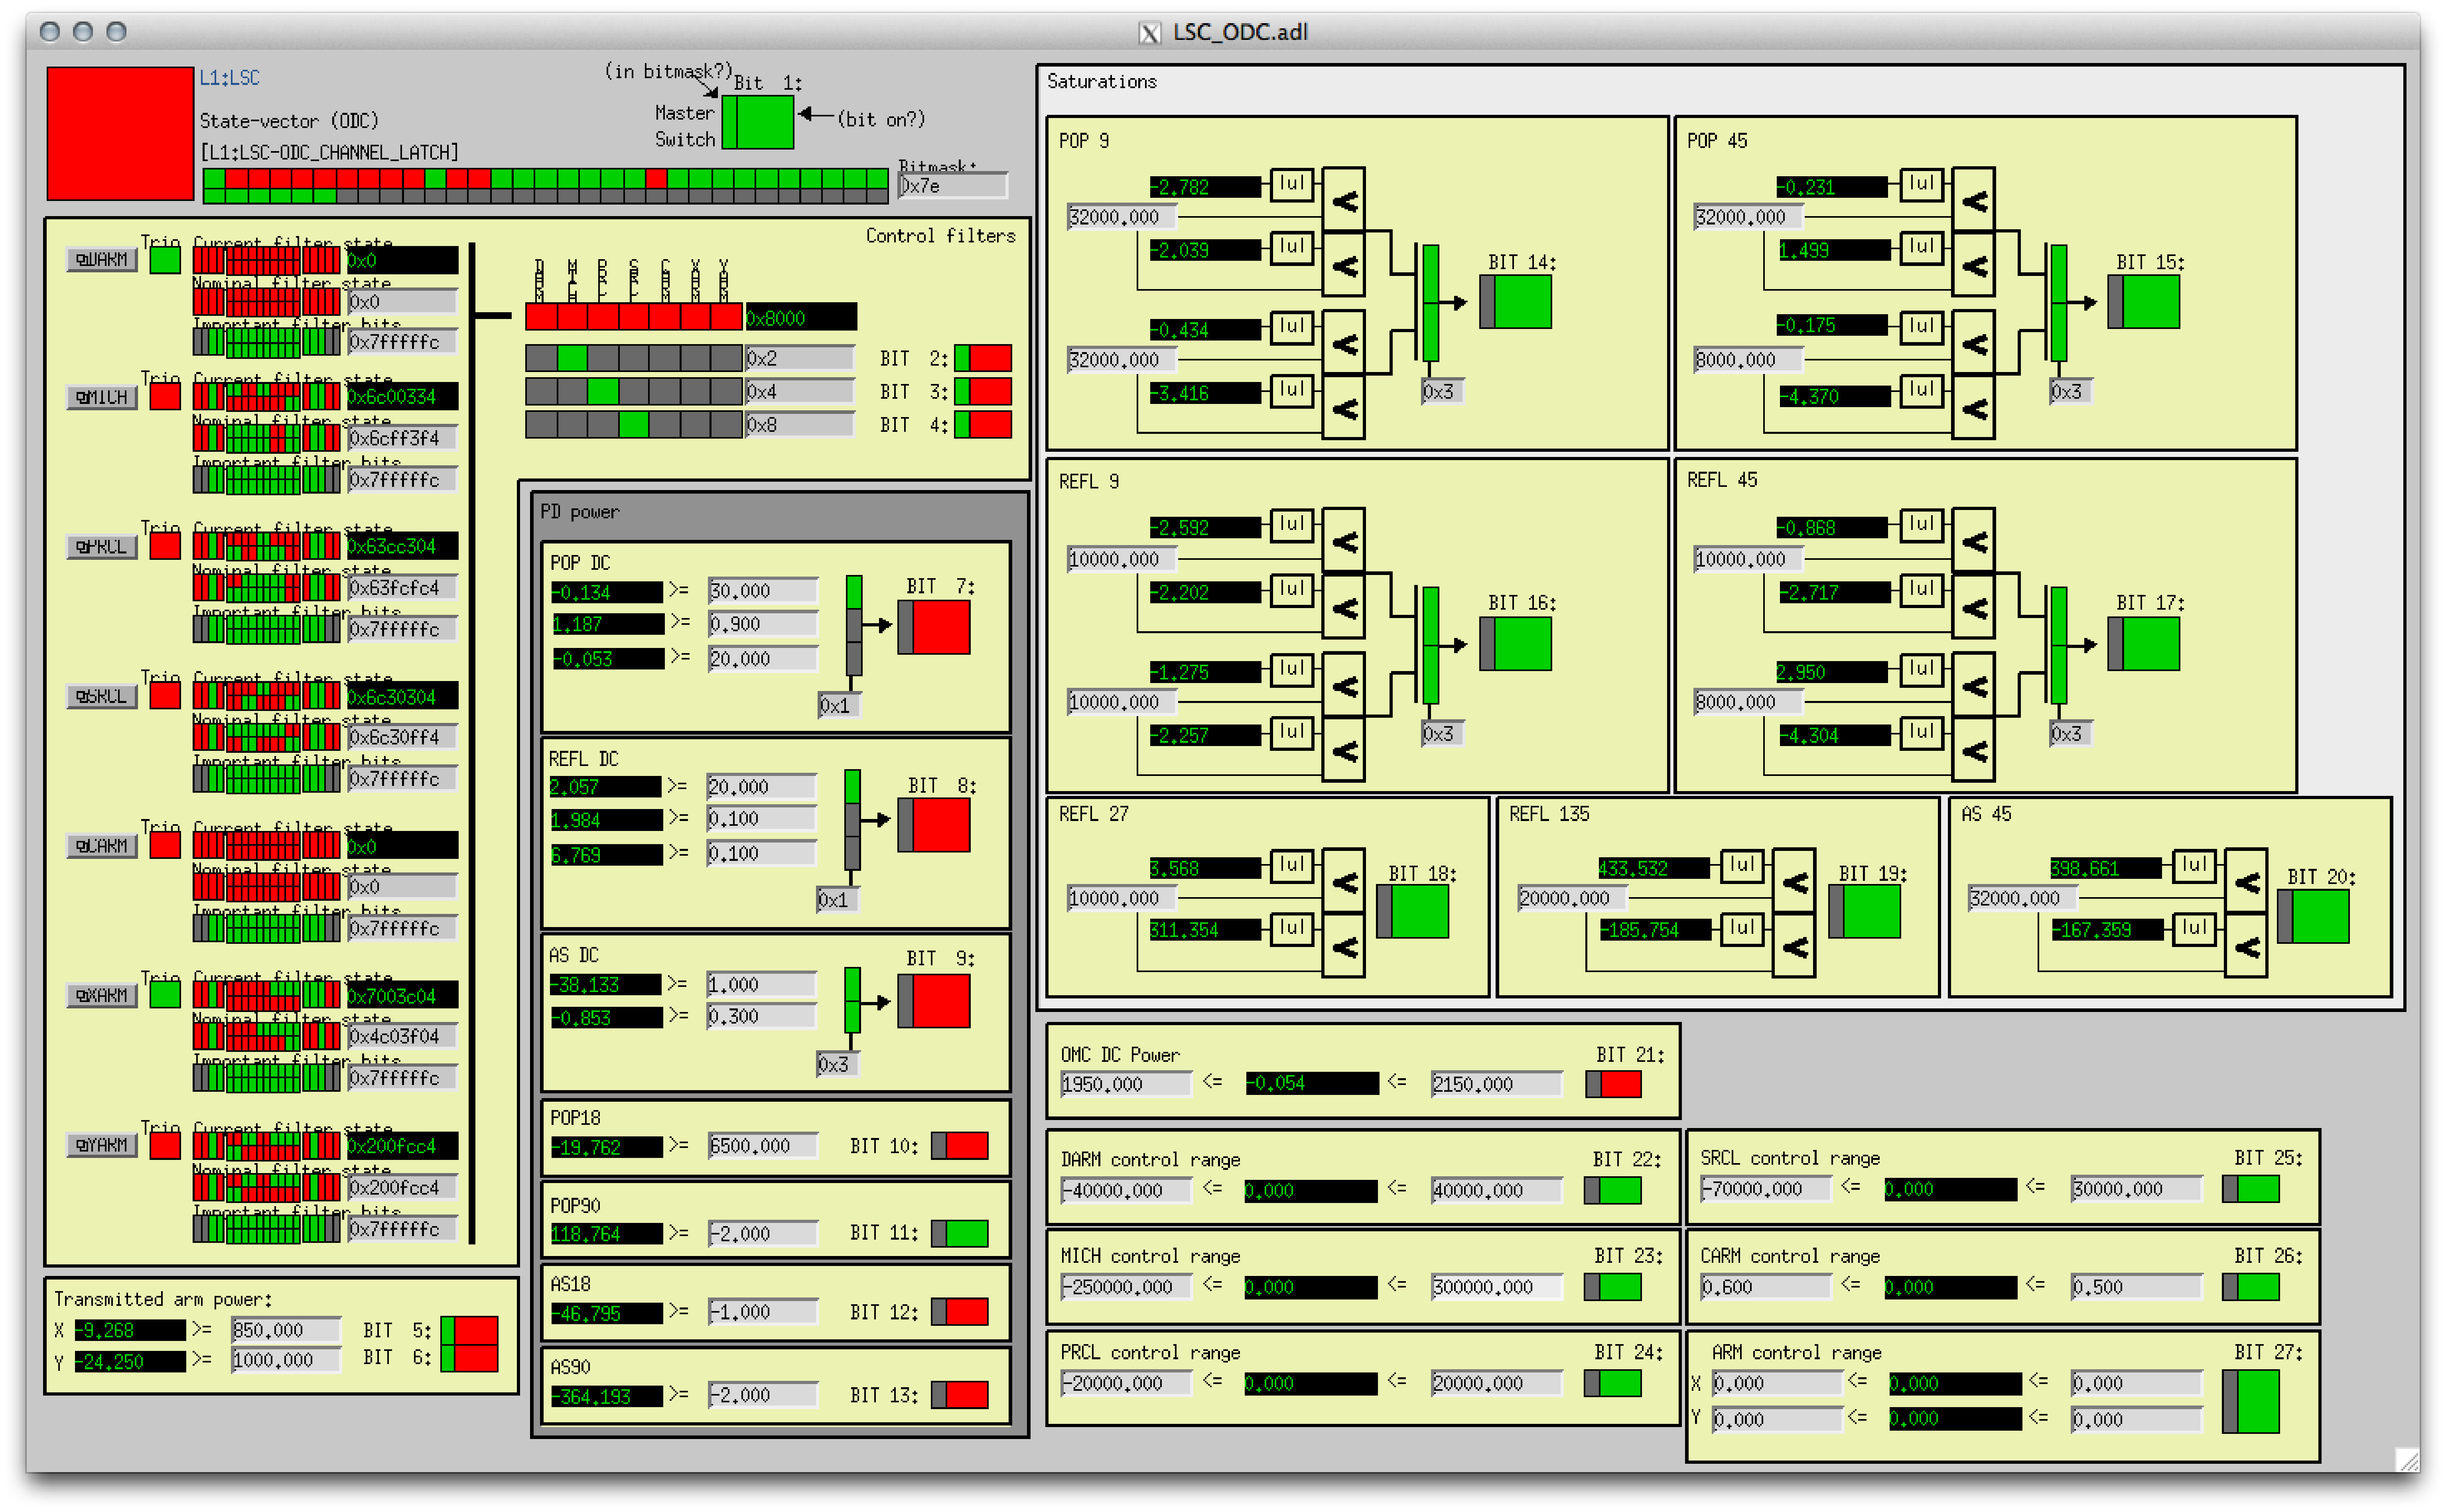
\includegraphics[width=\textwidth]{figures/ODC/LSC_screen}
\caption[LSC ODC Overview Screen]{MEDM screen used to control LSC ODC}
\end{figure}\label{fig:lsc-odc}

\subsection{Summary pages}
I made them

\section{Alignment Sensing and Control}

\subsection{Alignment locking basics}

Describe what I did

\subsection{Online Detector Characterization}

Also made an ASC ODC

\subsection{MEDM screens}

Figure \ref{fig:asc-odc} shows the ASC ODC overview screen in MEDM.

\begin{figure}[ht!]
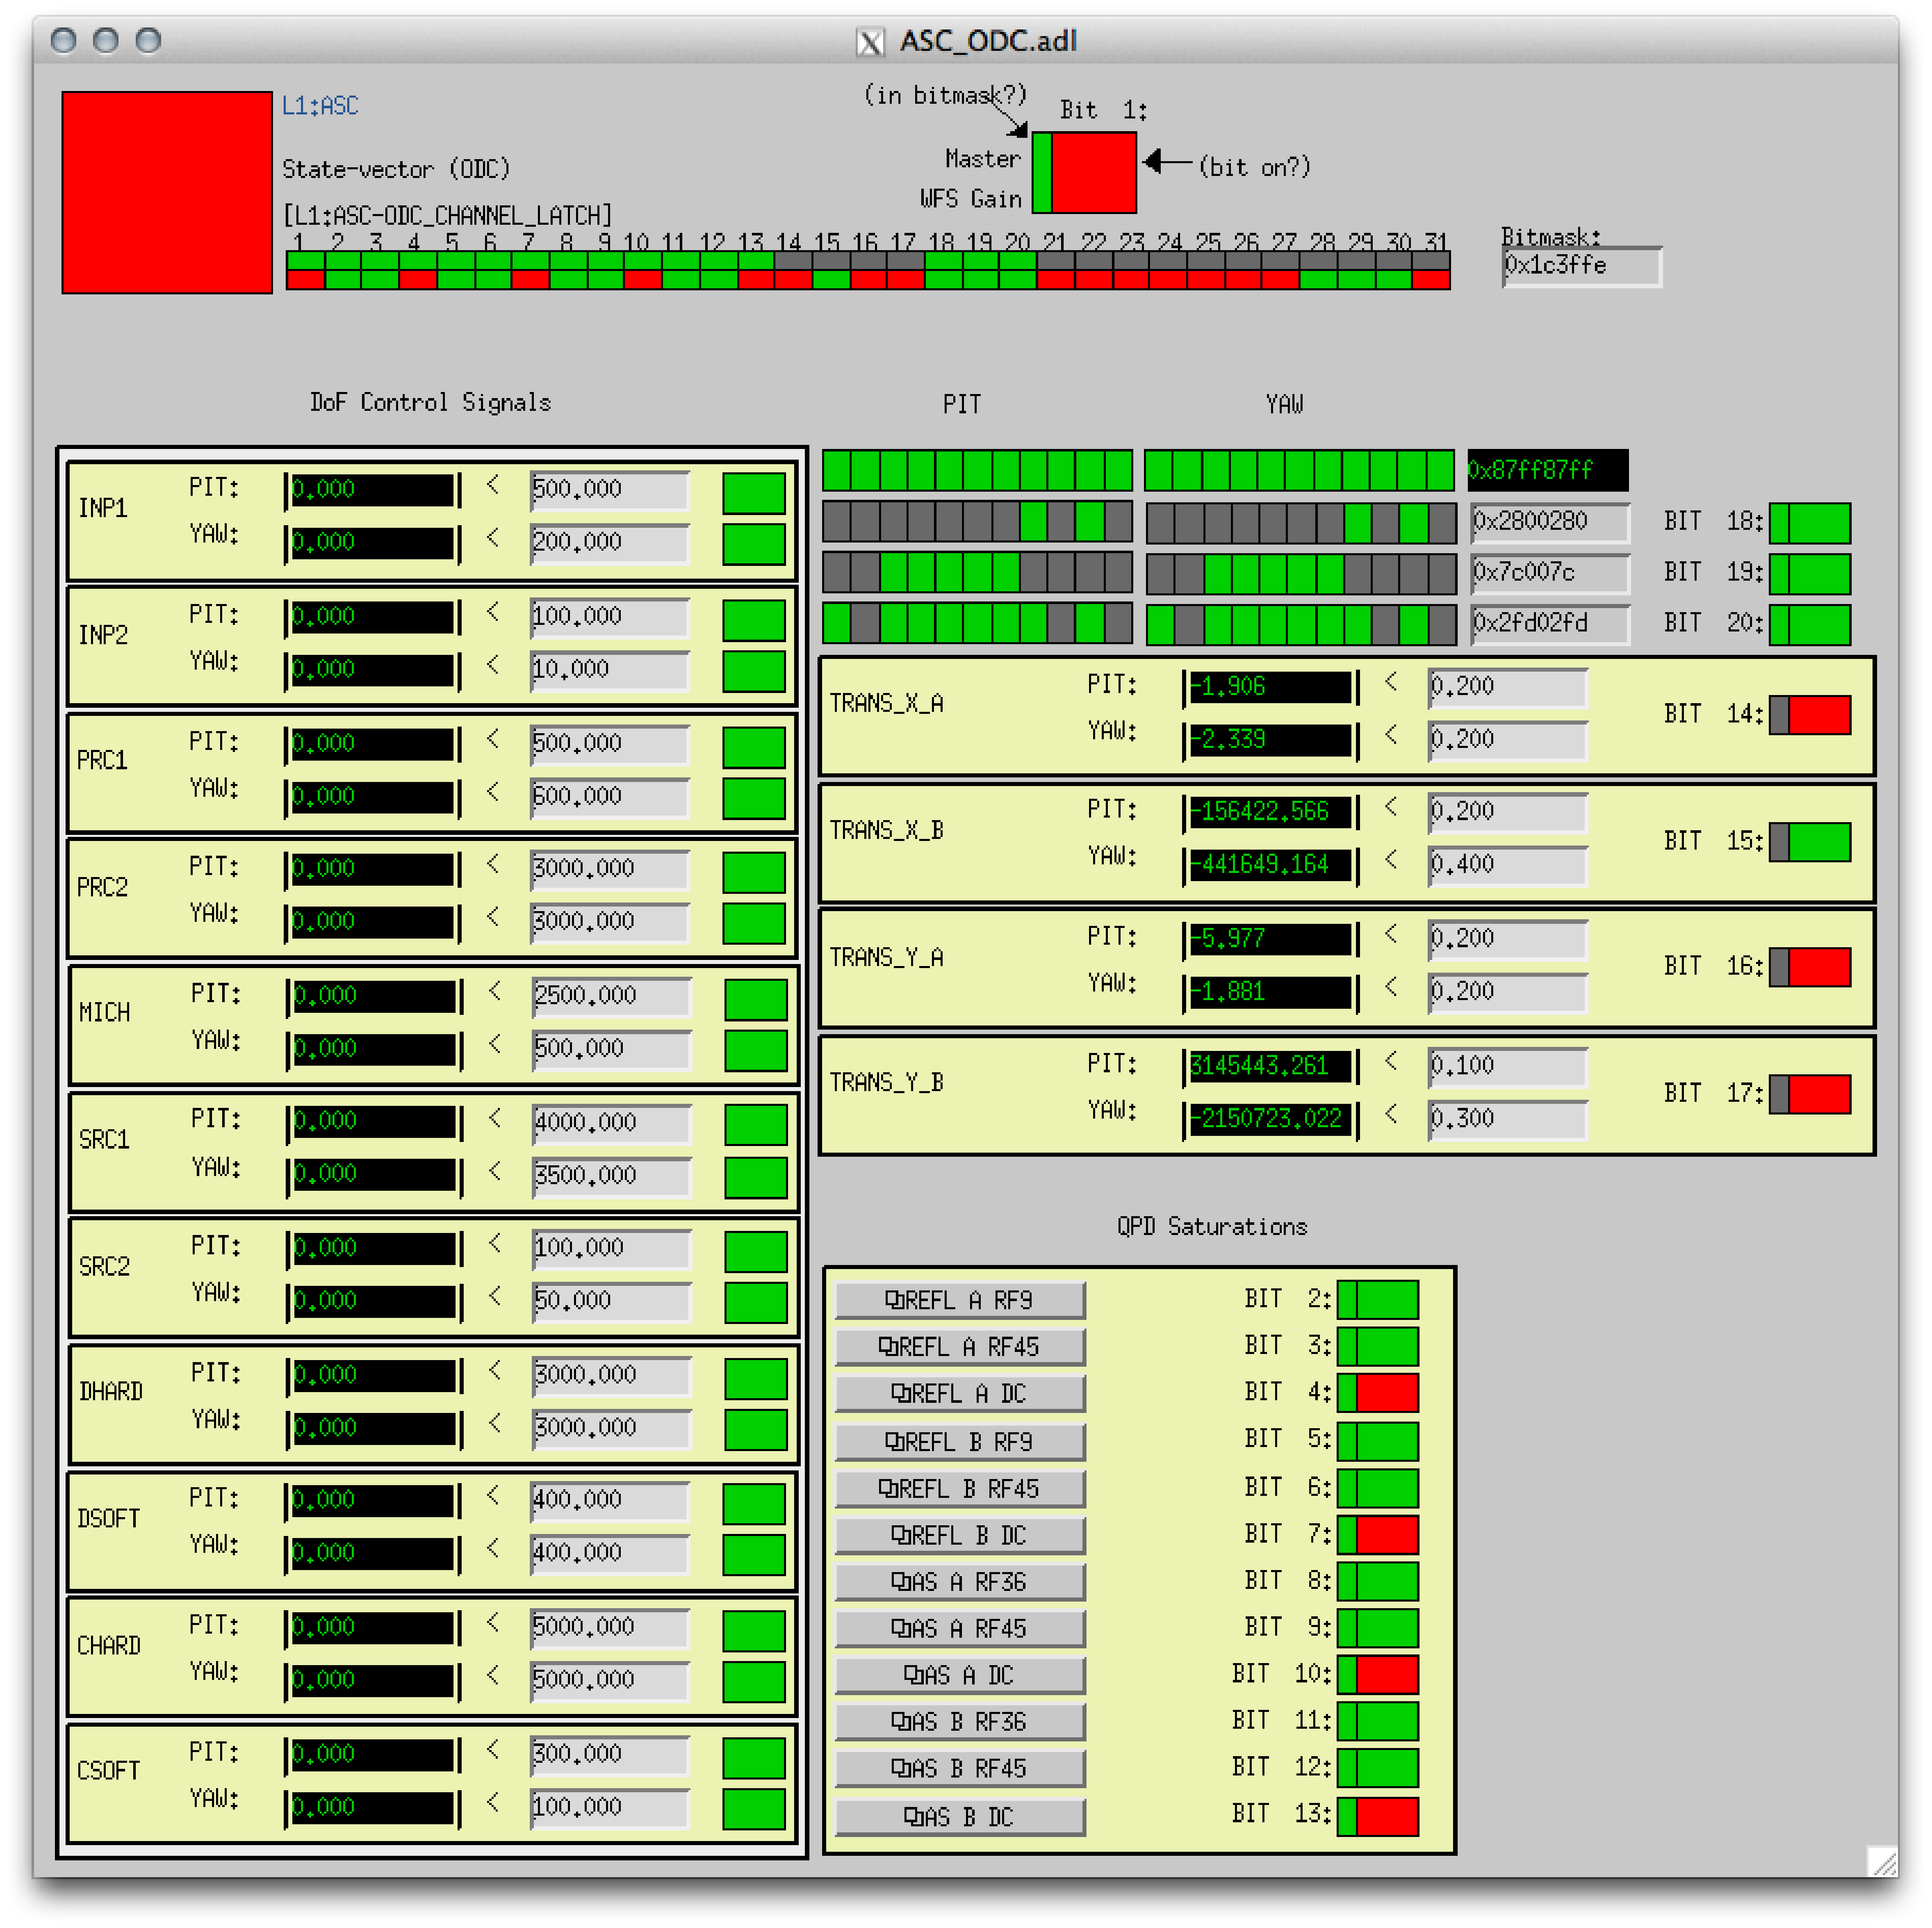
\includegraphics[width=\textwidth]{figures/ODC/ASC_screen}
\caption[ASC ODC Overview Screen]{MEDM screen used to control ASC ODC}
\end{figure}\label{fig:asc-odc}

Figure \ref{fig:odc-pd-screen} shows a photodiode monitor screen in the ASC ODC. 

\begin{figure}[ht!]
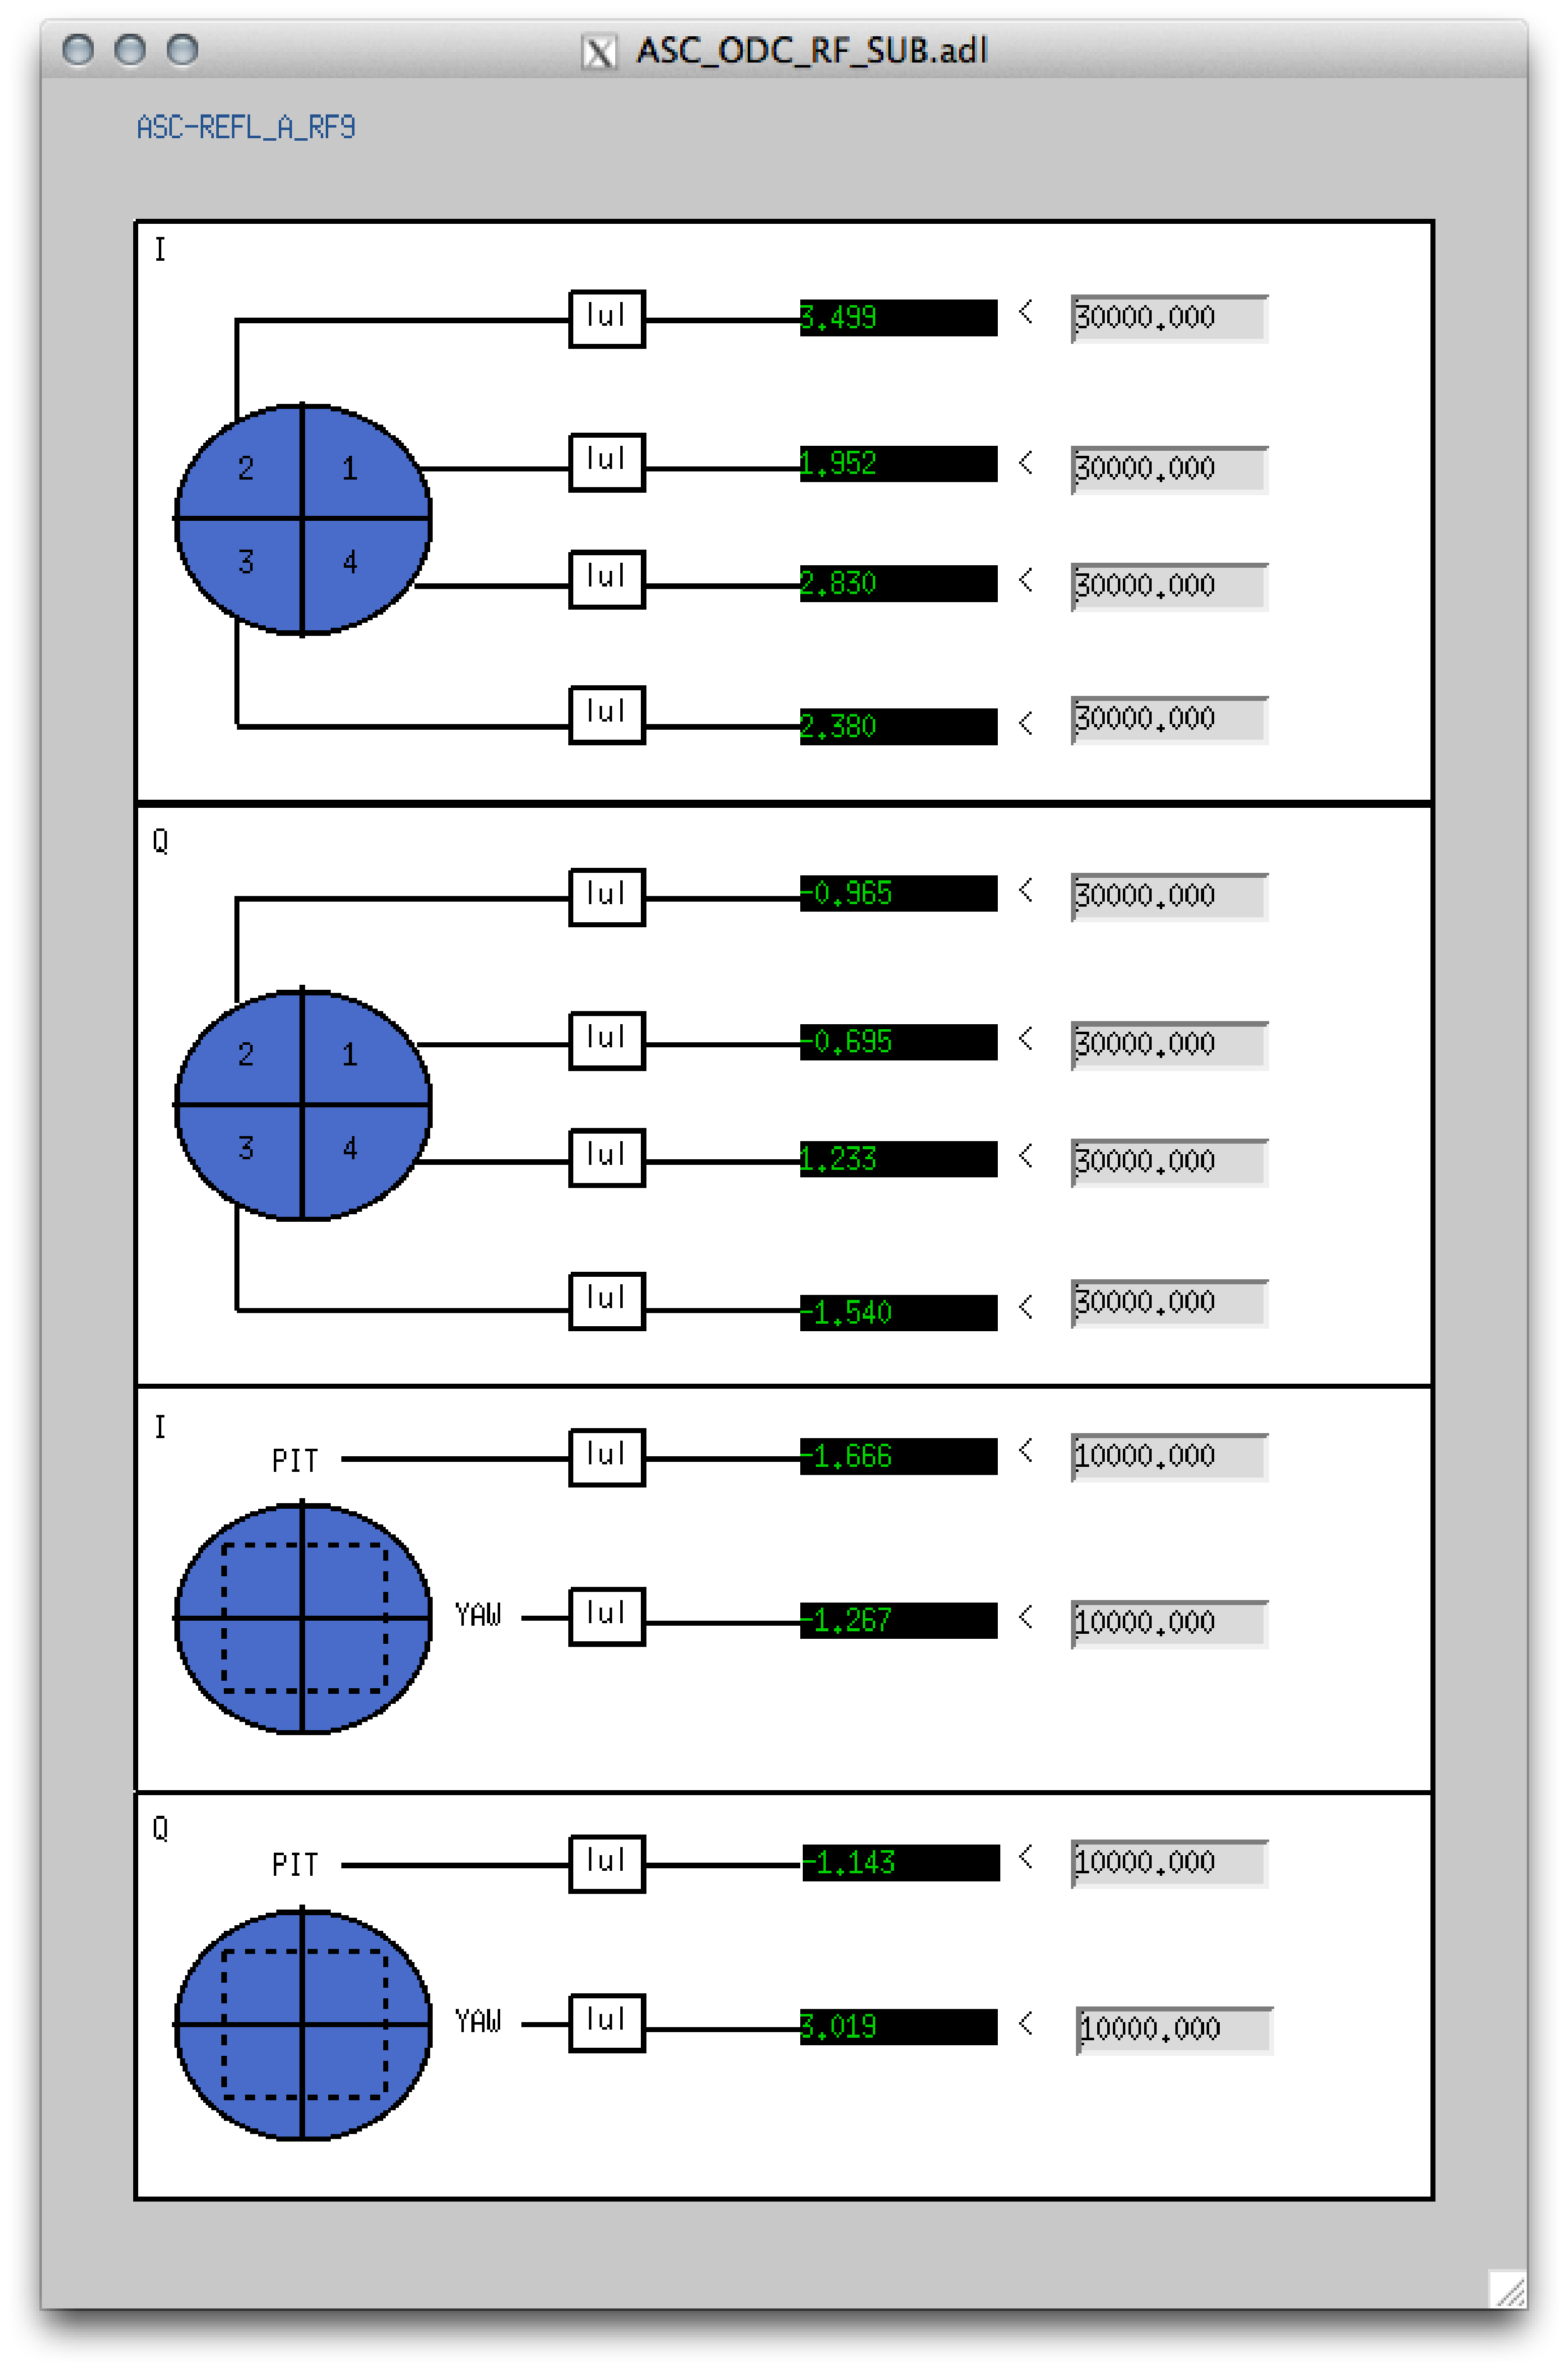
\includegraphics[width=\textwidth]{figures/ODC/PD_screen}
\caption[ASC ODC Photodiode Monitor in MEDM]{ODC monitor for ASC photodiode in MEDM}
\end{figure}\label{fig:odc-pd-screen}

\subsection{Summary pages}
I made them

\section{ODC Results}

We've been able to use ODC for a few interesting things.

\subsection{MICH ODC as a witness of RF45 glitches}

The ODC channel built to monitor the Michelson (MICH) pitch degree of freedom 
was used to generate vetoes used in O1 analyses. Throughout O1, the H1 
interferometer was prone to a glitch mechanism driven by malfunctions in 
RF electronics used to generate frequency sidebands on the carrer beam. 
These RF sidebands are used to control auxiliary degrees of freedom in the 
interferometer, including the length of the small Michelson interferometer 
formed by the beamsplitter and the two ITMs. When the RF electronics glitched, 
the error signals of these cavities would also glitch, causing excess motion 
in the auxiliary degrees of freedom that was witnessed by ODC monitors set 
up to monitor the control signal of the MICH alignment control loops. 

Figure \ref{fig:mich-odc-example} 
shows the correlation between the witness channel for this ODC channel 
and glitches in $h(t)$ as identified by Omicron. Figure \ref{subfig:mich-odc-timeseries} 
shows a timeseries the control signal of the MICH pitch control loop. The ODC threshold, 
set at a value of 250 for this particular channel, is indicated by the green dotted 
line. Any time the control signal crosses this threshold, a segment is created to 
indicate that the control loop is not in a nominal operating state. Figure 
\ref{subfig:mich-odc-omicron} shows the $h(t)$ Omicron triggers over the same 
duration. When the MICH pitch control point has a high variance, for example 
in the first 1.5 hours of the plot, there is an 
overall increase in the rate of high SNR Omicron triggers, indicating that 
this ODC channel is witnessing alignment fluctuations that couple into the 
output of the interferometer. 

\begin{figure}[ht!]%
\subfloat[]{
  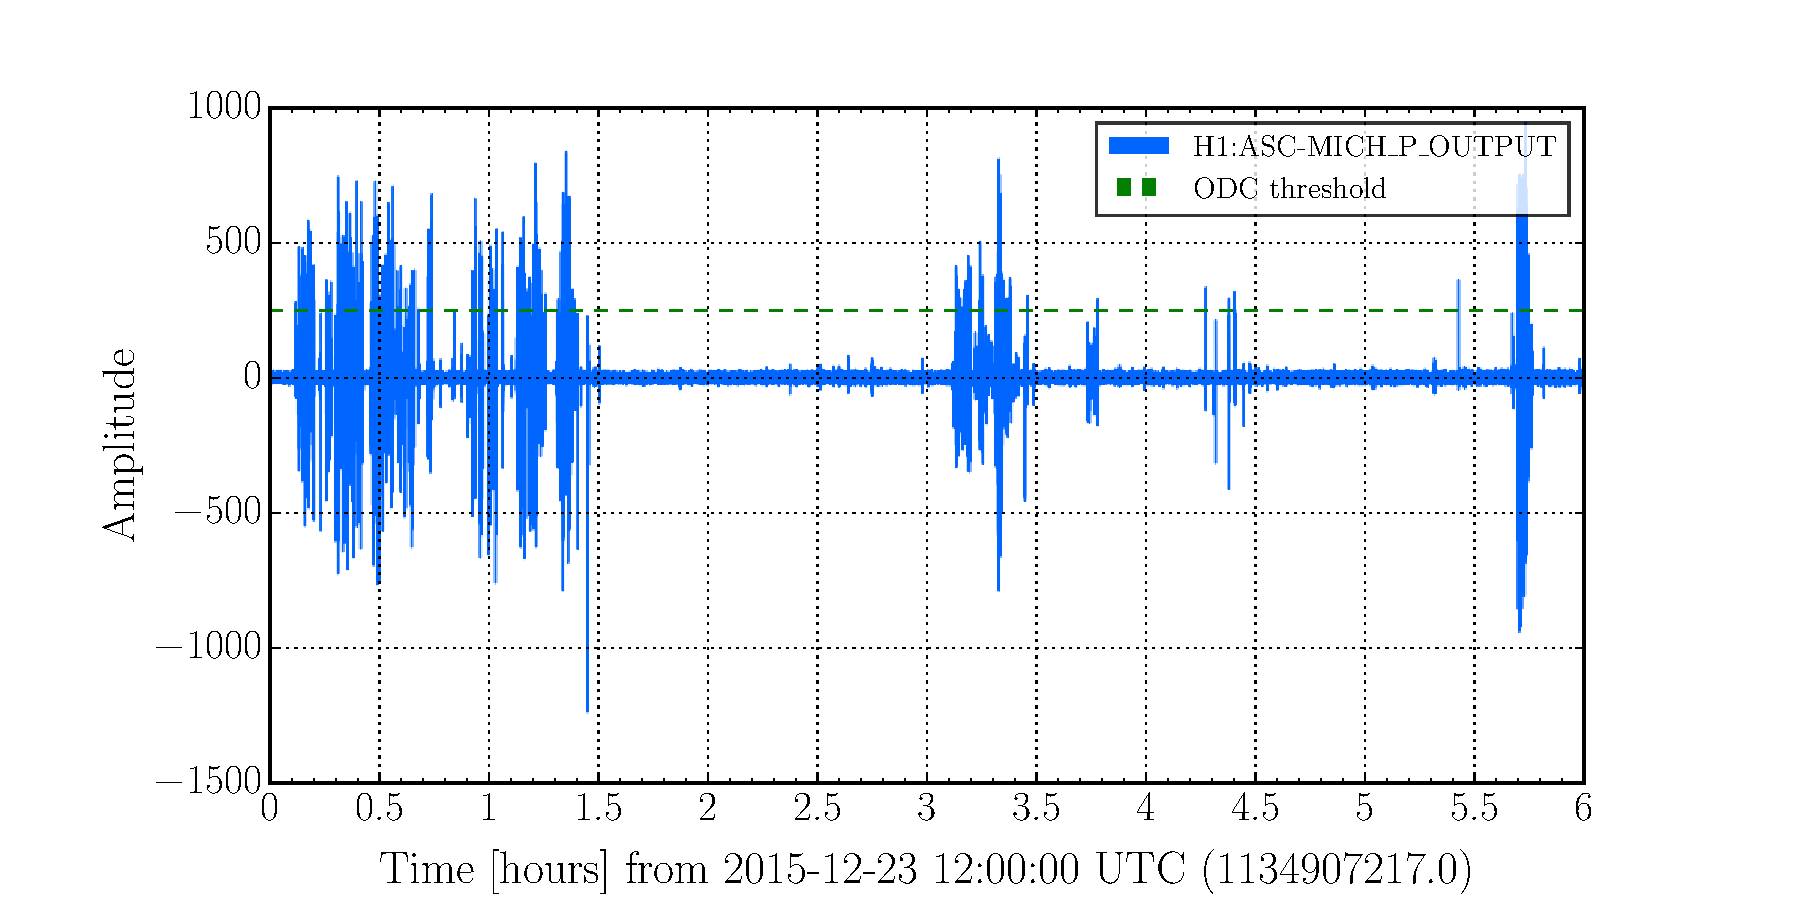
\includegraphics[width=\textwidth]{figures/detchar/MICH_P_OUTPUT_ODC}
  \label{subfig:mich-odc-timeseries}
  }

\subfloat[]{
  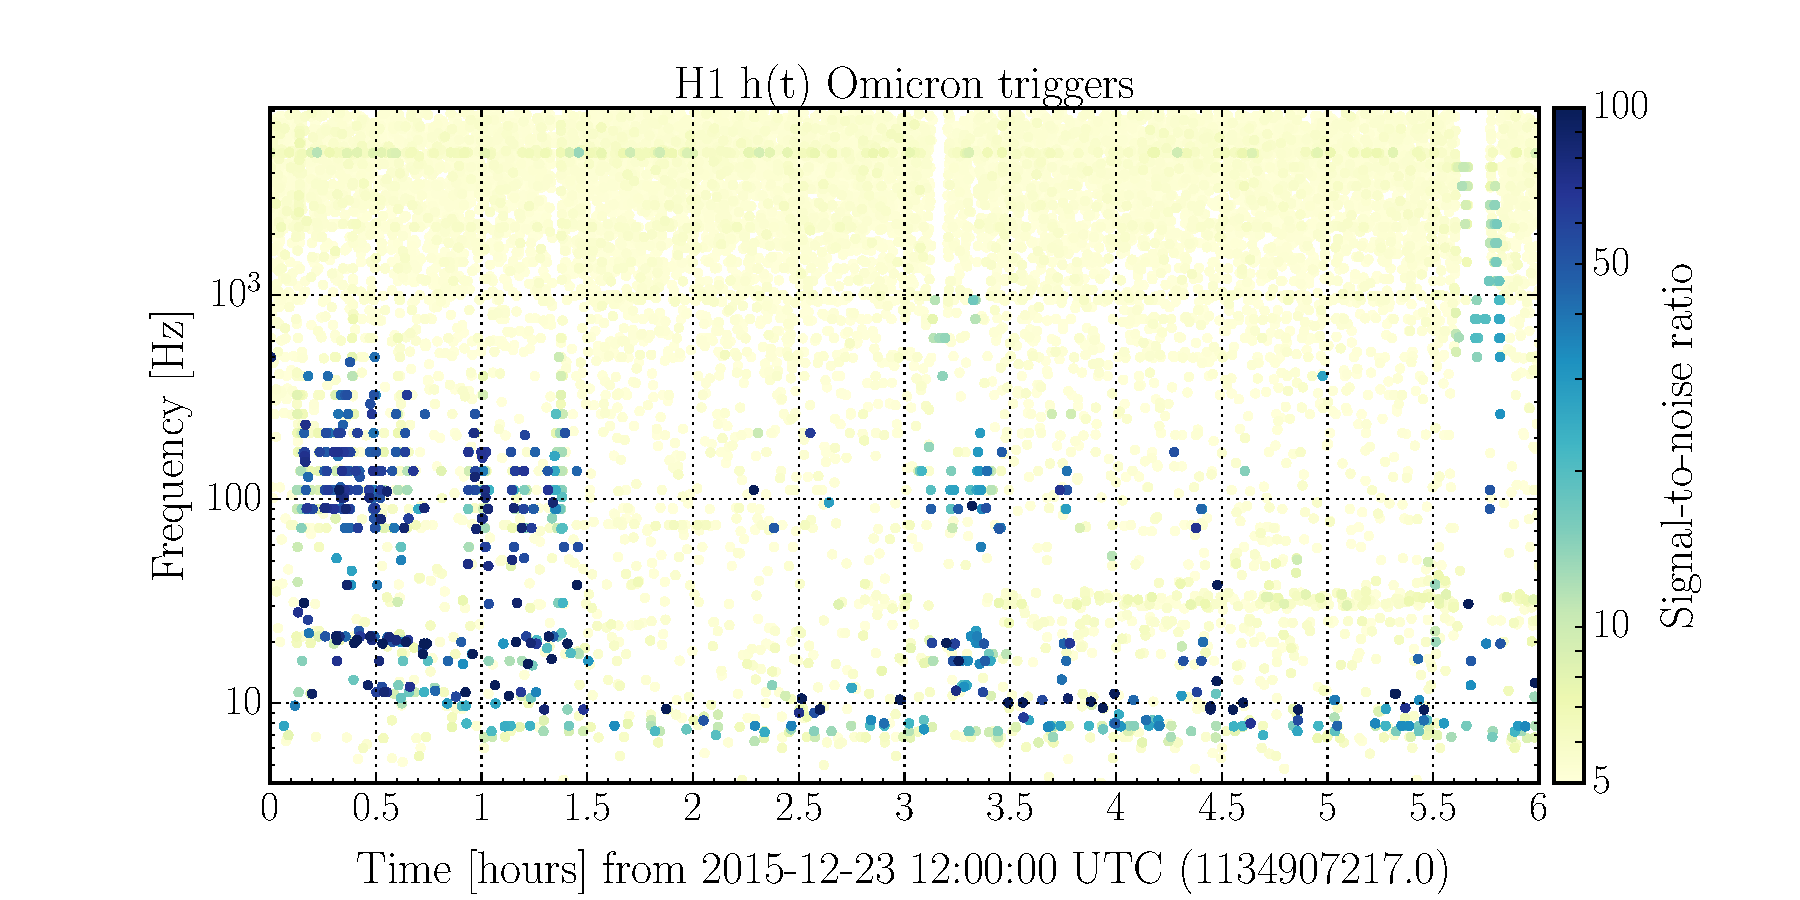
\includegraphics[width=\textwidth]{figures/detchar/Omicron_MICH_ODC}
  \label{subfig:mich-odc-omicron}
  }
\caption[ODC threshold on MICH pitch]{%
         An example of an ODC channel witnessing RF electronics issues, which %
         manifested as angular fluctuations in the vertex degrees of freedom %
         at H1. Figure \ref{subfig:mich-odc-timeseries} shows the ODC threshold %
         marking fluctuations in the MICH pitch degree of freedom. Figure %
         \ref{subfig:mich-odc-omicron} shows the associated Omicron triggers from %
         $h(t)$ at the same time. The storms of loud triggers between 10 - 400 Hz %
         are coincident with times flagged by this ODC monitor.}
\end{figure}\label{fig:mich-odc-example}

This coupling can be quantified using the veto evaluation tool (VET). The 
segments generated by this ODC channel are very efficient at vetoing high SNR 
Omicron triggers. VET reports that these segments veto Omicron triggers with SNR 
$>$ 8 with an efficiency:deadtime ratio of 47.16, indicating that these segments 
veto a large number of high SNR Omicron triggers with very little deadtime. These 
veto segments were included in the veto definer files that were distributed to 
the CBC and Burst searches in O1. 

\subsection{Using alignment flags as a pre-lockloss flag}

Tuned thresholds seem to be decent lockloss predictors.

Measure difference between segment end times and locklosses, histogram values


